
{
\textbf{The Binomial Probability Distribution}
\begin{itemize}
\item  The number of independent trials is denoted $n$.
\item  The probability of a `success' is $p$
\item  The expected number of `successes' from $n$ trials is $E(X) = np$
\end{itemize}
}
%---------------------------------------------------------------------------%
{
\textbf{Characteristics of a Poisson Experiment}
A Poisson experiment is a statistical experiment that has the following properties:
\begin{itemize}
\item  The experiment results in outcomes that can be classified as successes or failures.
\item  The average number of successes (m) that occurs in a specified region is known.
\item  The probability that a success will occur is proportional to the size of the region.
\item  The probability that a success will occur in an extremely small region is virtually zero.
\end{itemize}
Note that the specified region could take many forms. For instance, it could be a length, an area, a volume, a period of time, etc.
}

%---------------------------------------------------------------------------%
{
\textbf{Probability Tables}
\begin{itemize}
\item  For some value $r$ the tables record the probability of $P(X \geq r)$.
\item  The Student is required to locate the appropriate column based on the parameter values for the distribution in question.
\item  A copy of the Murdoch Barnes Tables will be furnished to the student in the End of Year Exam. The Tables are not required for the first mid-term exam.
\item  Knowledge of the sample space, partitioning of the sample points, and the complement rule are advised.
\end{itemize}
}
%---------------------------------------------------------------------------%


{
\textbf{Binomial Distribution : Using Tables}
It is estimated by a particular bank that 25\% of credit card customers pay only the minimum amount due on their monthly credit card bill and do not pay the total amount due. 50 credit card customers are randomly selected.
\begin{enumerate}
\item  (3 marks)What is the probability that 9 or more of the selected customers pay only the minimum amount due?
\item  (3 marks) What is the probability that less than 6 of the selected customers pay only the minimum amount due?
\item  (3 marks)What is the probability that more than 5 but less than 10 of the selected customers pay only the minimum amount due?
\end{enumerate}

}

{
\textbf{Binomial Distribution : Using Tables}
Demonstration on Blackboard re: how to use tables in class.
\begin{enumerate}
\item  $P(X \geq 9) = 0.9084$
\item  $P(X < 6) = 1- P(X \geq 6) =1 - 0.9930 = 0.0070$
\item  $P(6 \leq X \leq 9) = P(X \geq 6) - P(X \geq 10) = 0.9930 - 0.8363 = 0.1567$
\end{enumerate}

}







%---------------------------------------------------------------------------------------------------------------%
%----R Code ----
%---------------------------------------------------------------------------------------------------------------%
n=60000
Y=numeric(n)
for ( i in 1:n){

X=floor(runif(100,1,7))
Y[i]=sum(X)
}

Y
hist(Y,breaks=seq(300,400,by=10),main=c("Totals of 100 Die Throws"),cex.lab=1.4,font.lab=2,xlab=c("Total Score"))

hist(Y,breaks=seq(300,400,by=20),main=c("Totals of 100 Die Throws"),cex.lab=1.4,font.lab=2,xlab=c("Total Score"))



Z=seq(1:n)
Y/Z

plot(Y/Z,type="l",col="red",main=c("Die Rolls: Running Average"),font.lab=2,ylab="Average Value", xlab=
" Number of Throws")
abline(h=3.5,col="green")


#####################################################

plot(Z,Z.y,pch=16,col="red",ylim=c(2.5,5.5),main=c("Variance"),font.lab=2,ylab=" ", xlab="X: Green  Y: Blue  Z: Red" )

points(Y,Y.y,pch=16,col="blue" )
points(X,X.y,pch=16,col="green" )
points(c(1000,1000,1000),c(3,4,5),pch=18,cex=1.2)
lines(c(1000,1000),c(2.75,5.25),lty=3)



n=100000
Y=numeric(n)
for ( i in 1:n){

X=floor(runif(100,1,7))
Y[i]=mean(X)
}

Y
hist(Y,breaks=seq(270,430,by=2),main=c("Mean of 100 Die Throws (n= 100,000)"),cex.lab=1.4,font.lab=2,xlab=c("Mean of 100 throws")) 

\newpage


%---------------------------------------------------------------------------------------------------------------%
%----R Code ----
%---------------------------------------------------------------------------------------------------------------%
n=60000
Y=numeric(n)
for ( i in 1:n){

X=floor(runif(100,1,7))
Y[i]=sum(X)
}

Y
hist(Y,breaks=seq(300,400,by=10),main=c("Totals of 100 Die Throws"),cex.lab=1.4,font.lab=2,xlab=c("Total Score"))

hist(Y,breaks=seq(300,400,by=20),main=c("Totals of 100 Die Throws"),cex.lab=1.4,font.lab=2,xlab=c("Total Score"))



Z=seq(1:n)
Y/Z

plot(Y/Z,type="l",col="red",main=c("Die Rolls: Running Average"),font.lab=2,ylab="Average Value", xlab=
" Number of Throws")
abline(h=3.5,col="green")


#####################################################

plot(Z,Z.y,pch=16,col="red",ylim=c(2.5,5.5),main=c("Variance"),font.lab=2,ylab=" ", xlab="X: Green  Y: Blue  Z: Red" )

points(Y,Y.y,pch=16,col="blue" )
points(X,X.y,pch=16,col="green" )
points(c(1000,1000,1000),c(3,4,5),pch=18,cex=1.2)
lines(c(1000,1000),c(2.75,5.25),lty=3)



n=100000
Y=numeric(n)
for ( i in 1:n){

X=floor(runif(100,1,7))
Y[i]=mean(X)
}

Y
hist(Y,breaks=seq(270,430,by=2),main=c("Mean of 100 Die Throws (n= 100,000)"),cex.lab=1.4,font.lab=2,xlab=c("Mean of 100 throws")) 

%---------------------------------------------------------------------------------------------------------------%
%----R Code ----
%---------------------------------------------------------------------------------------------------------------%

{
\begin{itemize}
\item  Binomial Coefficients / The Choose Operator
\item  Definition: The Probability Mass Functions (pmf)
\item  Binomial Distribution : Example
\end{itemize}
}
{
\textbf{Binomial Coefficients}

In the last class, we came across binomial coefficients. Informally, binomial coefficients are the number of ways $k$ items can be selected from a group of $n$ items. 
The binomial coefficient indexed by n and k is usually written as $^nC_k$ or
\[ {n \choose k}\].
$C$ is colloqially known as the ``choose operator".

\[ {n \choose k} = \frac{n!}{k! \times (n-k)!} \]

(We call the operator the choose operator. We will use both notations interchangeably.)


%---------------------------------------------------------------------------%
{
\textbf{Probability Mass Function}
(Formally defining something mentioned previously)
\begin{itemize} \item  a probability mass function (pmf) is a \textbf{\emph{function}}
that gives the probability that a discrete random variable is exactly equal to some
value.
\[P(X=k)\]
\item  The probability mass function is often the primary means of defining a discrete
probability distribution
\item  It is conventional to present the probability mass function in the form of a table.
\item  The p.m.f of a value $k$ is often denoted $f(k)$.
\end{itemize}
}
%--------------------------------------------------------------------------------------%
{
\textbf{Probability Tables}
In the \textbf{Sulis} workspace there are two important tables used for this part of the course.


This class will feature a demonstration on how to read those tables.
\begin{itemize}
\item  The Cumulative Binomial Tables (Murdoch Barnes Tables 1)
\item  The Cumulative Poisson Tables (Murdoch Barnes Tables 2)
\end{itemize}

Please get a copy of each as soon as possible.

}

%---------------------------------------------------------------------------%
{
\textbf{Probability Tables}
\begin{itemize}
\item  For some value $r$ the tables record the probability of $P(X \geq r)$.
\item  The Student is required to locate the appropriate column based on the parameter values for the distribution in question.
\item  A copy of the Murdoch Barnes Tables will be furnished to the student in the End of Year Exam. The Tables are not required for the first mid-term exam.
\item  Knowledge of the sample space, partitioning of the sample points, and the complement rule are advised.
\end{itemize}
}
%---------------------------------------------------------------------------%


{
\textbf{Binomial Distribution : Using Tables}
It is estimated by a particular bank that 25\% of credit card customers pay only the minimum amount due on their monthly credit card bill and do not pay the total amount due. 50 credit card customers are randomly selected.
\begin{enumerate}
\item  (3 marks)What is the probability that 9 or more of the selected customers pay only the minimum amount due?
\item  (3 marks) What is the probability that less than 6 of the selected customers pay only the minimum amount due?
\item  (3 marks)What is the probability that more than 5 but less than 10 of the selected customers pay only the minimum amount due?
\end{enumerate}

}

{
\textbf{Binomial Distribution : Using Tables}
Demonstration on Blackboard re: how to use tables in class.
\begin{enumerate}
\item  $P(X \geq 9) = 0.9084$
\item  $P(X < 6) = 1- P(X \geq 6) =1 - 0.9930 = 0.0070$
\item  $P(6 \leq X \leq 9) = P(X \geq 6) - P(X \geq 10) = 0.9930 - 0.8363 = 0.1567$
\end{enumerate}

}


%------------------------------------------------------------------%
{
\textbf{Binomial Distribution: Expected Value and Variance}


If the random variable X has a binomial distribution with parameters n
and p, we write
\[ X \sim B(n,p) \]

Expectation and Variance
If $X \sim B(n,p)$, then:

\begin{itemize}
\item  Expected Value of X : $E(X) = np$
\item  Variance of X : $Var(X) = np(1-p)$
\end{itemize}

Suppose n=3 and p=0.5 
Then $E(X) = 1.5$ and $V(X) = 0.75$.

Remark: Referring to the expected value and variance may be used to validate
the assumption of a binomial distribution.

}


%---------------------------------------------------------------------%

\textbf{The Cumulative Distribution Function}
\begin{itemize}
\item  The Cumulative Distribution Function, denoted $F(x)$, is a common way that the probabilities
of a random variable (both discrete and continuous) can be summarized.
\item  The Cumulative Distribution Function, which also can be
described by a formula or summarized in a table, is defined as:
\[F(x) = P(X \leq x) \]
\item  The notation for a cumulative distribution function, F(x), entails using a capital
"F".  (The notation for a probability mass or density function, f(x), i.e. using a lowercase "f". The notation is not interchangeable.
\end{itemize}



\section{Useful Results for Discrete Random Variables}
%---------------------------------------------------------------------%



\textbf{Useful Results}
(Demonstration on the blackboard re: partitioning of the sample space, using examples on next slide)
\begin{itemize}
\item $P(X \leq 1) = P(X=0) + P(X=1)$
\item $P(X \leq r) = P(X=0)+ P(X=1) + \ldots P(X= r)$
\item $P(X \leq 0) = P(X=0)$
\item $P(X = r) = P(X \geq r ) - P(X \geq r + 1)$
\item \textbf{Complement Rule}: $P(X \leq r-1) = P(X < r) = 1 - P(X \geq r)$
\item \textbf{Interval Rule}:$ P(a \leq X \leq  b)= P(X \geq a) - P(X \geq b + 1).$
\end{itemize}
For the binomial distribution, if the probability of success is greater than 0.5, instead of
considering the number of successes, to use the table we consider
the number of failures.

%---------------------------------------------------------------------%



%--------------------------------------------------%
\itemIn a newspaper on average 1 in 10 000 characters is incorrectly printed. Suppose the paper contains 50 000 characters. Calculate the exact probability that 
\begin{itemize}
\item[(i)]no printing errors are made
\item[(ii)]at least 3 errors are made
\end{itemize}
Using the appropriate approximation, estimate these two probabilities. 

\textbf{Binomial Example }

Suppose a die is tossed 5 times. What is the probability of getting exactly 2 fours?

\textbf{Solution:}

This is a binomial experiment in which \begin{itemize}\item a success is defined as an outcome of `4'. \item the number of trials is equal to $n=5$, \item the number of successes is equal to $k=2$,\item the number of failures is equal to 3, \item  the probability of success on a single trial is 1/6, \item  the probability of failure on a single trial is 5/6.\end{itemize}

\textbf{Binomial Example }

Therefore, the probability of getting exactly 2 fours is:

\[P(X=2) = ^5C_2 \times (1/6)^2 \times (5/6)^3 = 0.161\]

Remark: $^5C_2 = 10$\\


\begin{center}
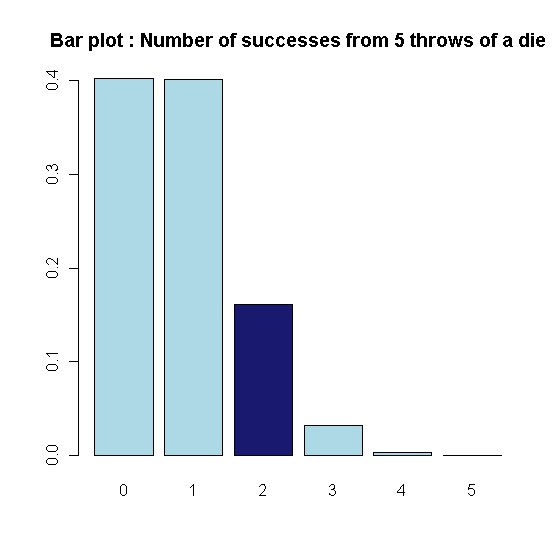
\includegraphics[scale=0.40]{images/3Bbarplot4}
\end{center}


\textbf{Remark} : The sum of the probabilities of each of the possible outcomes (i.e. no fours, one four etc) is equal to one.
\[P(X=0) + P(X = 1) + \ldots + P(X=5) = 1 \]

%\begin{figure}
%\centering
%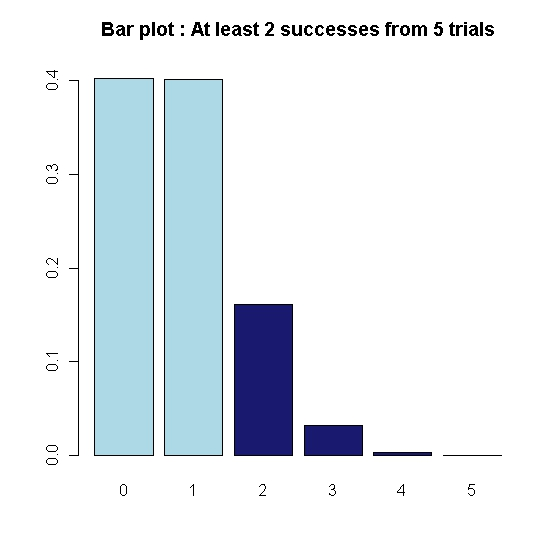
\includegraphics[width=0.7\linewidth]{images/3Bbarplot5}
%\caption{}
%\label{fig:3Bbarplot5}
%\end{figure}


\textbf{Binomial Example: At least two successes}
\begin{itemize}
\item Suppose we were asked to find the probability of \textbf{\emph{at least}} 2 fours.
\item Can you suggest the most efficient way of computing this?
\item Suggestion: Compute $P(X=0)$ and $P(X = 1)$.
\item Together these probabilities are the complement probability of what we require.
\item $P(X \geq 2) = 1 - ( P(X=0) + P(X = 1))$.
\item (We will continue with this in future classes).
\end{itemize}

%=================================================================================%


\item \textbf{Binomial Example: Sample Problem}

Suppose there are twelve multiple choice questions in an English class quiz. Each question has five possible answers, and only one of them is correct. Find the probability of having four or less correct answers if a student attempts to answer every question at random.



\textbf{Solution:}
Since only one out of five possible answers is correct, the probability of answering a question correctly by random is $1/5=0.2$. We can find the probability of having exactly 4 correct answers by random attempts as follows.(Blackboard. Correct Answer is 13.29\%)
%\begin{verbatim}
%> dbinom(4, size=12, prob=0.2)
%[1] 0.1329
%\end{verbatim}


\item \textbf{ Binomial Example 1 }
(Revision from Last Class)\\
Suppose a die is tossed 5 times. What is the probability of getting exactly 2 fours?

\textbf{Solution:} This is a binomial experiment in which the number of trials is equal to 5, the number of successes is equal to 2, and the probability of success on a single trial is 1/6 or about 0.167. 
\\
\bigskip
Therefore, the binomial probability is:

\[P(X=2) = ^5C_2 \times (1/6)^2 \times (5/6)^3 = 0.161\]

\textbf{ Binomial Example 2 }
Suppose there is a container that contains 6 items.  The probability that any one of these items is defective is 0.3. Suppose all six items are inspected. 
\begin{itemize}
\item What is the probability of 3 defective components?
\item What is the probability of 4 defective components?
\end{itemize}

\[ P(3\text{ defects}) = f(3) = P(X = 3) = {6\choose 3}0.3^3 (1-0.3)^{6-3} = 0.1852 \]
\[ P(4\text{ defects}) = f(4) = P(X = 4) = {6\choose 4}0.3^4 (1-0.3)^{6-4} = 0.0595 \]


\item \textbf{Binomial Distribution: Example 2}

\begin{itemize}
\item Let the number of containers be the number of independent trials is $n=100$.
\item A success may be defined as a defective component.
\item The probability of a success is approximate $p=0.10$. (The probability of ``failure" is $1-p=0.9$).
\item The expected number of defective components is $np=10$, which concurs with our observed data.
\item The variance is computed as \[np(1-p) = 100 \times 0.1 \times 0.9 = 9\]
\item The observed standard deviation is 3 units, i.e. a variance of 9 square units.
\item Yes the binomial distribution is useful in this case.
\end{itemize}

\item \noindent \textbf{ Binomial Example 1}

Suppose a die is tossed 5 times. What is the probability of getting exactly 2 fours?

Solution: This is a binomial experiment in which the number of trials is equal to 5, the number of successes is equal to 2, and the probability of success on a single trial is 1/6 or about 0.167. Therefore, the binomial probability is:

\[P(X=2) = ^5C_2 \times (1/6)^2 \times (5/6)^3 = 0.161\]

\end{enumerate}
%============================================================ %
%====================================================================%
\section{Question 3 : Binomial Distribution}

\begin{itemize}
\item 10\% of intended passengers dont show up. Each flight holds 50 people.

\item Binomial distribution with parameters n=50 and p = 0.1

\item From Murdoch Barnes Table 1 (third page of tables at back of book )
\end{itemize}
\begin{itemize}
\item a) What is the probability that six people or more fail to show up.

\[P(X=6) =0.3839\]

\item b) Less than three people fail to show up (i.e. X=0,1 or 2)

\[P(X < 3) = 1- P(X3) =    1 - 0.8883  = 0.1117\] [ANS]


\item c) More than 2 but less than 8   (i.e. X = 3,4,5,6,7)

This is equal to \[P(X=3) - P(X=8) = 0.8883 -0.1221 =  0.7662\]

\end{itemize}


\noindent \textbf{ Binomial Example 1}

Suppose a die is tossed 5 times. What is the probability of getting exactly 2 fours?

Solution: This is a binomial experiment in which the number of trials is equal to 5, the number of successes is equal to 2, and the probability of success on a single trial is 1/6 or about 0.167. Therefore, the binomial probability is:

\[P(X=2) = ^5C_2 \times (1/6)^2 \times (5/6)^3 = 0.161\]



\section{Binomial Distribution: Worked Example}
Suppose a gambler is playing a simple coin flip game. 
The gambler does not know that the coin has been tampered with such that the probability of a Head is 47\%.

Suppose the gamble plays this coin flip game nine times. 
What is the probability that he wins precisely 3 times.
%----------------------------------------------%





\section{Binomial Distribution}

MCQ questions  - 25\% chance of getting a single question right at random.

number of questions is 10

Binomial parameter values n=10, p = 0.25

X number of correct answers


\[P(X=7) = 0.0035 \]       [00.35\%]



\section{Poisson Questions}
%==================================%








\subsection{Question D01  - Poisson Example}
A motor dealership which specializes in agricultural machinery sells on vehicle every 2 days, on average

In this question the unit period is one day. The company expects to sell, on average, 0.5 vehicles every day.
The Poisson mean $m$ is therefore 0.5.

$P(X \geq 1)$

Go to your Poisson tables, and search for the $m=0.5$ column.
We are interested in the probability of \textbf{exactly} one vehicle sold on a particular day.
From the tables we can easily work out P($X \geq 1$), but this is probability of one or more vehicles being sold.
This is not the same thing.
\[P(X \geq 1) = P(X =1) + P( X=2) + P(X=3) + \ldots
P(X \geq 1) = P(X=1) + P(X \geq 2)\]
From tables
$P(X \geq 1)$
$P(X \geq 2)$

Six day working week?
our unit period is now six days.
How many vehicles do we expect to sell in 6 days?
answer = 3
$m=3$

P($X\geq 4$)

\begin{eqnarray}
e^{-6/5} = 0.3011942
e^{-4/5} = 0.449329
e^{-5/5} = 0.3678794
\end{eqnarray}









%---------------------------------------------------%

(c)XYZ Ltd supplies motherboards to Dell.  You are a production manager with Dell.  There is a constant probability of 0.4 that a board will be defective.  You select 100 boards at random.  Using the log tables for the binomial distribution what is the probability that

\begin{itemize}
\item[(i)] 0 boards will be defective?
\item[(ii)] 2 or more boards will be defective?
\item[(iii)]5 or less boards will be defective?
\end{itemize}
% (6 marks)
(d)Use the normal approximation to the binomial to answer (i), (ii) and (iii) in part (c) above.
%(6 marks

\begin{enumerate}



%------------------------------------------------------------------------------------%
\end{enumerate}
\section{Geometric Distribution}

\itema) Suppose X has a geometric distribution with parameter p. From the standard interpretation of the geometric distribution, conditioning on whether X=1 or not and using the memoryless property of the geometric distribution
\begin{enumerate}[(i)]
\item calculate E(X)
\item calculate Var(X). [Hint: first calculate E(X2)].
\end{enumerate}


\section{Exponential}

\item Suppose X has an Exp(λ) distribution.
i)Derive E(X) and Var(X). [Use the fact that limx->∞ xk e-λx = 0, for any positive integer k].
ii)Using induction, show that the k-th moment of X is given by k!/λk .
iii)       Show that X has the memoryless property.



\item The average lifespan ppf a laptop is 5 year. You may assume that the lifespan of laptop computers follows an exponential distribution.

\begin{enumerate}
\item What is the probability that the lifespan of the laptop will be at least 6 years.
\[e^{-6/5} = 0.3011942\]
\item What is the probability that the lifespan of the laptop will not exceed 4 years.
\[e^{-4/5} = 0.449329\]
\item What is the probability that the lifespan of the laptop will be between 5 years and 6 years.
\[e^{-5/5} = 0.3678794\]
\end{enumerate}


\section{Normal}



\begin{enumerate}






\end{enumerate}

\end{document}
